% !TeX spellcheck = es_ES
\documentclass[titlepage]{article}
\usepackage[letterpaper, margin=2.5cm]{geometry}
\usepackage[utf8]{inputenc}
\usepackage[spanish]{babel}
\usepackage{listings}
\usepackage{url}
\usepackage{float}
\usepackage{graphicx} 
\usepackage{amsmath}
\usepackage{color}
\usepackage{algorithm}
\usepackage{algorithmic} 

\usepackage[nottoc,notlot,notlof]{tocbibind}
\definecolor{dkgreen}{rgb}{0,0.6,0}
\definecolor{gray}{rgb}{0.5,0.5,0.5}
\definecolor{mauve}{RGB}{253,151,31}
\definecolor{deepred}{RGB}{249,38,114}

\lstset{frame=tb,
  language=Python,
  aboveskip=3mm,
  belowskip=3mm,
  showstringspaces=false,
  columns=flexible,
  numbers=left,
  stepnumber=1,
  basicstyle={\small\ttfamily},
  numberstyle=\tiny\color{gray},
  keywordstyle=\color{blue},
  commentstyle=\color{dkgreen},
  stringstyle=\color{mauve},
  breaklines=true,
  breakatwhitespace=true,
  tabsize=2,
  morekeywords={self, append},
  emph={Transicion, __init__, True, False, __str__, AFN, AFD, Analizador},
  emphstyle=\color{deepred}
}

\makeatletter
\def\BState{\State \hskip-\ALG@thistlm}
\makeatother

%opening
\title{Reporte: Práctica 3}
\author{Barrera Pérez Carlos Tonatihu \\ Profesor: Saucedo Delgado Rafael Norman \\ Compiladores \\ Grupo: 3CM6 }

\begin{document}

\maketitle
\tableofcontents
\newpage
\section{Introducción}
El transformar un autómata no determinista a uno determinista surge de la necesidad de modelar dicho autómata computacionalmente. Esto debido a que la implementación de un AFN debido a los múltiples movimientos que podría realizar en un estado con un sólo símbolo
\begin{figure}[H]
        \begin{center}
        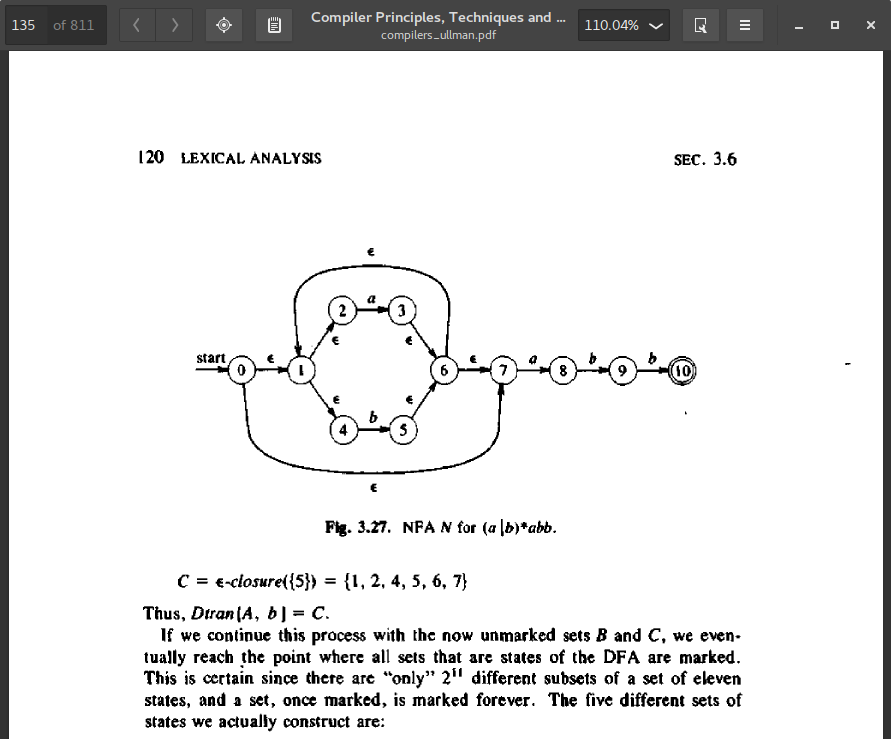
\includegraphics[width=10cm]{AFN.png}
        \caption{AFN que reconoce el lenguaje $(a|b)^{*}abb$.}
        \label{fig:AFN}
        \end{center}
    \end{figure}
Es por esto que se utiliza el siguiente algoritmo (construcciones de subconjuntos) para pasar de un AFN a un AFD \cite{compis}. Este algoritmo se basa en que cada estado en el AFD es igual a un subconjunto de estados del AFN. Para construir estos subconjuntos se utilizan las siguientes funciones.
\begin{itemize}
	\item \emph{cerradura-$\epsilon(T)$}. Esta función recibe un conjunto de estados $T$ del AFN y retorna el conjunto de estados que se pueden obtener al hacer transiciones épsilon. Por ejemplo, aplicar esta función sobre el estado inicial del autómata de la figura \ref{fig:AFN} produciría lo siguiente: cerradura-$\epsilon(\{0\}) = \{0, 1, 2, 4, 7\}$.
	
	\item \emph{mover$(T, a)$}. Regresa el conjunto de estados que se pueden obtener al realizar transiciones con el símbolo $a$ sobre el conjunto de estados $T$ del AFN. Un ejemplo de esto es que si se aplica esta función sobre el conjunto del ejemplo anterior se produciría lo siguiente: mover$(\{0, 1, 2, 4, 7\}, a) = \{3, 8\}$.
\end{itemize}
Este conjunto de funciones se ejecutaran las veces que sean necesarias hasta que se obtenga el nuevo conjunto de estados del AFD. Esto se ve de forma más clara en el siguiente pseudocódigo.
\begin{algorithm}
	\caption{Obtención de subconjuntos}
	\begin{algorithmic} 
		\STATE Agregar $cerradura$-$\epsilon($Inicial del AFN$)$ a $E$
		\FOR{cada $ e $ en $E$}
		\FOR{cada $ simbolo $ en el alfabeto del $AFN$}
		\STATE Agregar $cerradura$-$\epsilon(mover(e, s))$
		\STATE Agregar transición $e \rightarrow cerradura$-$\epsilon(mover(e, s))$ con símbolo $s$
		\ENDFOR
		\ENDFOR
		\STATE El inicial del $AFD$ es $cerradura$-$\epsilon($Inicial del AFN$)$
		\STATE Los finales del $AFD$ contienen finales del $AFN$
	\end{algorithmic}
\end{algorithm} 

\begin{figure}[H]
        \begin{center}
        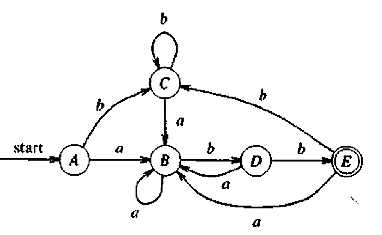
\includegraphics[width=10cm]{AFD.png}
        \caption{AFD que reconoce el mismo lenguaje que el AFN de la figura \ref{fig:AFN}.}
        \label{fig:AFD}
        \end{center}
    \end{figure}
\section{Desarrollo}
La siguiente clase contiene los métodos necesarios para transformar un AFN en un AFD basados en el algoritmo anterior.
\begin{lstlisting}
from automata.automatas import AFD

# Clase para poder etiquetar los nuesvos estados de manera mas facil
class Subconjunto:
	def __init__(self, estados, etiqueta):
		self.estados = estados
		self.etiqueta = etiqueta


class Transformacion:
	def __init__(self, AFN):
		self.lista = list()
		self.AFN = AFN
		self.AFD = AFD()
		self.etiqueta = 'A' # Para etiquetar los estados AFD
	
	def convertir_automata(self):
		self.AFD.alfabeto = self.AFN.alfabeto
		self.AFD.alfabeto.remove('e')
		estado = self.cerradura_epsilon(self.AFN.estado_inicial)
		actual = Subconjunto(estado, self.etiqueta)
		self.lista.append(actual)
		pendientes = list()
		pendientes.append(actual)
		agregar = True
		self.etiqueta = chr(ord(self.etiqueta) + 1)
		nuevo = None
		while len(pendientes) > 0:
			actual = pendientes.pop()
			for simbolo in self.AFD.alfabeto:
				estados = self.cerradura_epsilon(self.mover(actual.estados, simbolo))
				agregar = True
				for i in self.lista:
					if i.estados == estados:
						agregar = False
						nuevo  = i
						break
				if agregar:
					nuevo = Subconjunto(estados, self.etiqueta)
					pendientes.append(nuevo)
					self.lista.append(nuevo)
					self.etiqueta = chr(ord(self.etiqueta) + 1)
				print("Transicion %s -> %s con: %s" % (actual.estados, nuevo.estados, simbolo))
				self.AFD.agregar_transicion(actual.etiqueta, nuevo.etiqueta, simbolo)
		
		# Obtenemos los estados finales e inicial
		for elemento in self.lista:
			if self.AFN.estado_inicial in elemento.estados:
				self.AFD.estado_inicial = elemento.etiqueta
			for final in self.AFN.estados_finales:
				if final in elemento.estados:
					self.AFD.estados_finales.add(elemento.etiqueta)
	
	# recibe un solo elemento o un conjunto de estados
	def cerradura_epsilon(self, estados):
		estados_epsilon = set()
		aux = list()
		if type(estados) is set:
			aux.extend(estados)
		else:
			aux.append(estados)
		for estado in aux:
			for t in self.AFN.transiciones:
				if t.caracter == 'e' and t.actual == estado and (t.siguiente not in aux):
					aux.append(t.siguiente)
		
		estados_epsilon.update(aux)
		return estados_epsilon
	
	# Obtiene los siguientes estados con base en un simbolo y un conjunto de entrada
	def mover(self, estados, simbolo):
		estados_aux = set()
		for estado in estados:
			for transicion in self.AFN.transiciones:
				if simbolo != 'e' and estado == transicion.actual and transicion.caracter == simbolo:
					estados_aux.add(transicion.siguiente)
		return estados_aux

\end{lstlisting}
\section{Resultados}
Para realizar las pruebas se utilizo la siguiente función. En donde lo primero que se hace es crear un AFN basado en las clases creadas en prácticas anteriores para después transformarlo y realizar pruebas con diversas cadenas sobre este nuevo autómata determinista
\begin{lstlisting}
def transformar_automata(self):
	print('Transformando AFN a AFD')
	automata = AFN()
	automata.agregar_alfabeto({'a', 'b'})
	
	automata.agregar_estado(0)
	automata.agregar_estado(1)
	automata.agregar_estado(2)
	automata.agregar_estado(3)
	automata.agregar_estado(4)
	automata.agregar_estado(5)
	automata.agregar_estado(6)
	automata.agregar_estado(7)
	automata.agregar_estado(8)
	automata.agregar_estado(9)
	automata.agregar_estado(10)
	
	automata.agregar_inicial(0)
	automata.agregar_finales({10})
	
	automata.agregar_transicion(0, 1, 'e')
	automata.agregar_transicion(1, 2, 'e')
	automata.agregar_transicion(1, 4, 'e')
	automata.agregar_transicion(0, 7, 'e')
	automata.agregar_transicion(2, 3, 'a')
	
	automata.agregar_transicion(4, 5, 'b')
	automata.agregar_transicion(3, 6, 'e')
	automata.agregar_transicion(5, 6, 'e')
	automata.agregar_transicion(6, 1, 'e')
	automata.agregar_transicion(6, 7, 'e')
	automata.agregar_transicion(7, 8, 'a')
	automata.agregar_transicion(8, 9, 'b')
	automata.agregar_transicion(9, 10, 'b')
	
	transformer = Transformacion(automata)
	print('Transformando el automata')
	transformer.convertir_automata()
	print()
	print('-Automata deterministico final:')
	print("Estado inicial %s" % transformer.AFD.estado_inicial)
	print("Estados finales %s" % transformer.AFD.estados_finales)
	print("Transiciones")
	for t in transformer.AFD.transiciones:
		print(t)
	
	print('Evaluacion de cadenas:')
	for n in range(5):
		cadena = input("-Ingresa una cadena: ")
		print("La cadena es:")
		if transformer.AFD.evaluar_cadena(cadena):
			print("Valida")
		else:
			print("No valida")
\end{lstlisting}
    \begin{figure}[H]
        \begin{center}
        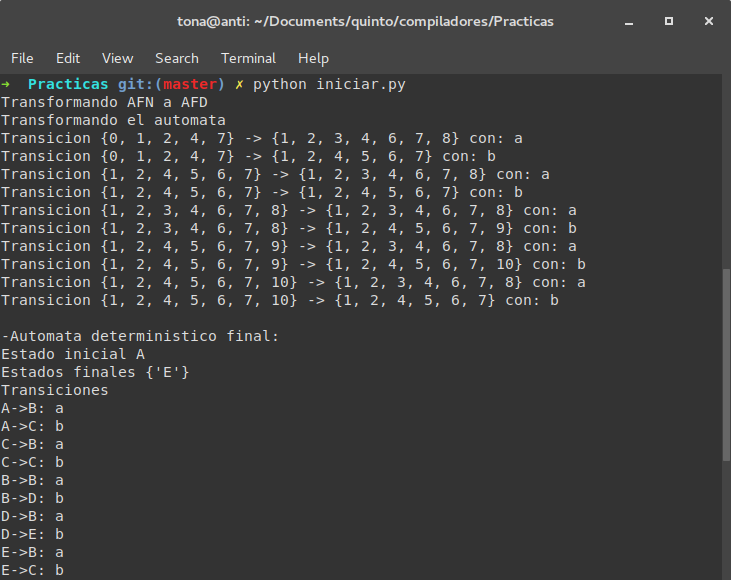
\includegraphics[width=\textwidth]{1.png}
        \caption{Estados como subconjuntos y estados re-etiquetados en el autómata determinista final.}
        \label{fig:creacion}
        \end{center}
    \end{figure}
    \begin{figure}[H]
        \begin{center}
        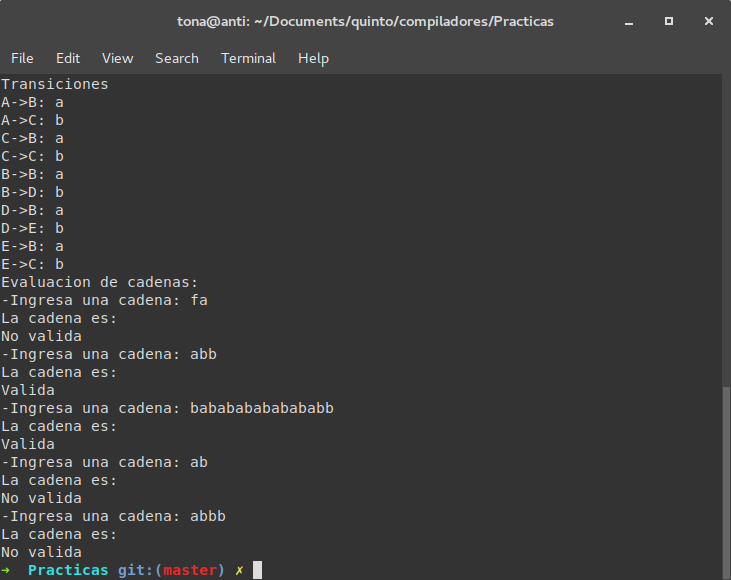
\includegraphics[width=\textwidth]{2.png}
        \caption{Pruebas realizadas sobre el autómata que se obtuvo a través de la transportación}
        \label{fig:pruebas}
        \end{center}
    \end{figure}
\section{Conclusiones}
    El desarrollo de esta práctica fue sencillo debido a que al tener los algoritmos ya definidos \cite{compis} solo se tuvo que modelar dichos algoritmos en un lenguaje orientado a objetos en este caso Python y después combinar esta práctica con la primer práctica realizada para la evaluación de cadenas. 
    
    Además, la realización de esta practica y las anteriores permitió entender la importancia que tienen las expresiones regulares y los autómatas en el análisis léxico de un compilador. Es por esto que para este punto la elaboración de un analizador léxico personal es posible.
    \bibliography{bibliografia} 
    \bibliographystyle{ieeetr}
\end{document}
